\documentclass[border=4pt]{standalone}\usepackage[utf8]{inputenc}\usepackage[T1]{fontenc}\usepackage{mathptmx}
\usepackage{tikz}
\usetikzlibrary{arrows.meta,positioning,calc,fit,backgrounds}
\tikzset{>={Stealth[length=2.2mm]}, font=\small,
 blk/.style={draw, line width=0.8pt, fill=white, align=center, inner sep=3pt, text width=#1, minimum height=1.1cm},
 blk/.default=3.0cm,
 iut/.style={fill=black!14},
 ext/.style={draw, dashed, line width=0.5pt, align=center, inner sep=3pt, text width=#1, minimum height=1.0cm, fill=white},
 ext/.default=2.6cm,
 grp/.style={draw=black!55, dashed, line width=0.5pt, fill=black!4, inner sep=7pt},
 glab/.style={font=\small\itshape, text=black!75, anchor=north west, inner sep=2pt},
 lab/.style={font=\footnotesize, inner sep=1.5pt, fill=white},
 pw/.style={line width=2.2pt, -{Stealth[length=2.6mm]}},
 dg/.style={line width=0.6pt},
 an/.style={line width=0.8pt, dashed},
 rf/.style={double, double distance=1.2pt, line width=0.4pt},
 cd/.style={line width=0.6pt, dotted}}

\begin{document}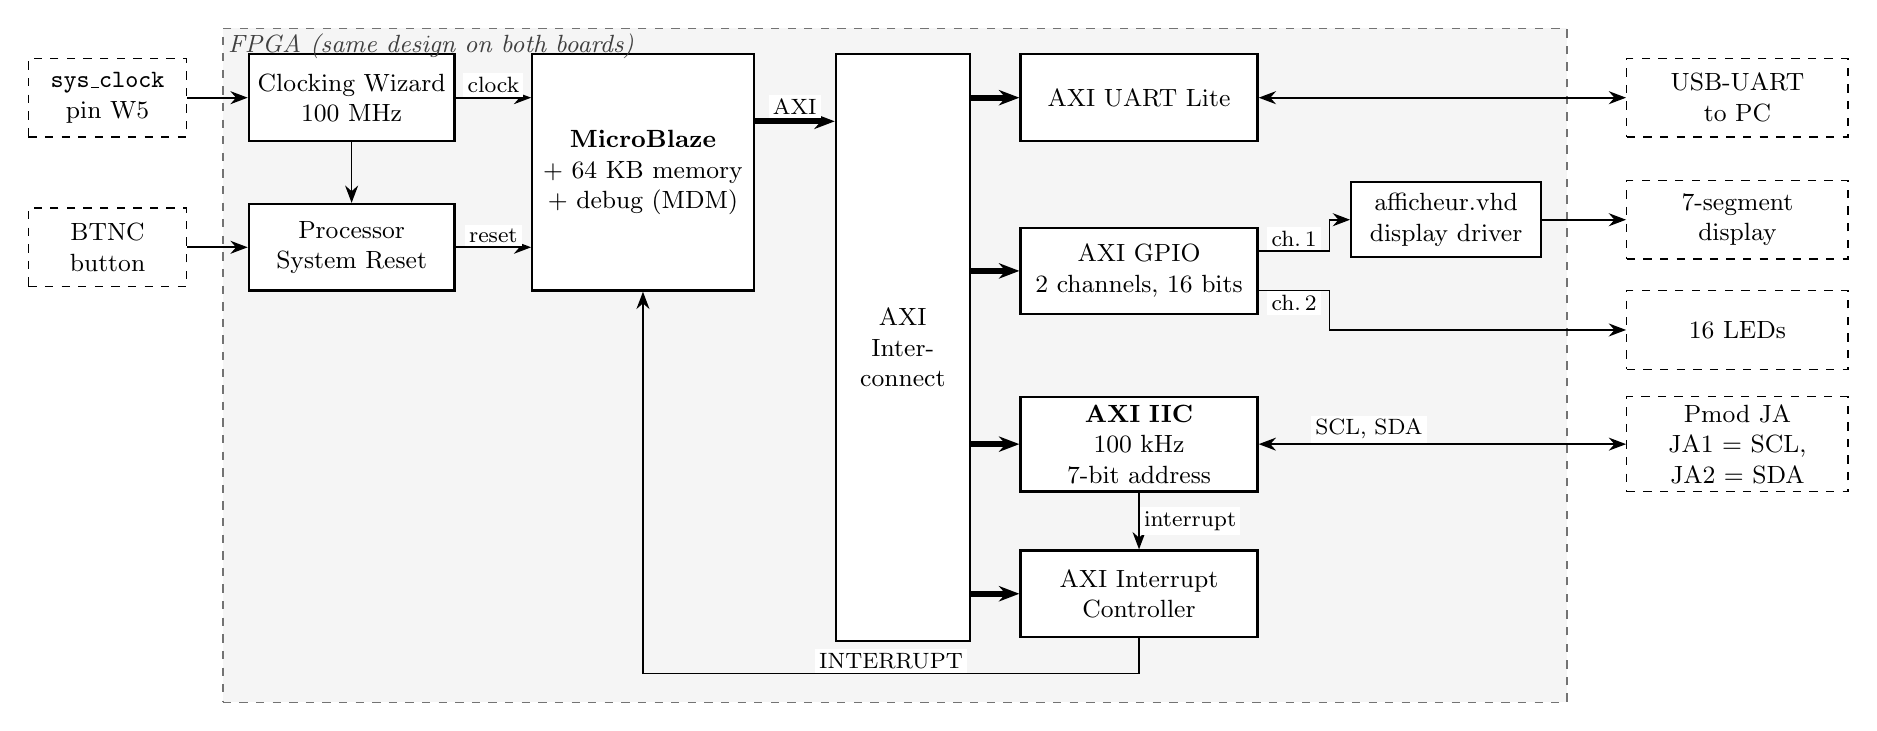
\begin{tikzpicture}
\node[blk=2.4cm] (clk) at (0,0) {Clocking Wizard\\100 MHz};
\node[blk=2.4cm] (rst) at (0,-1.9) {Processor\\System Reset};
\node[ext=1.8cm] (sys) at (-3.1,0) {\texttt{sys\_clock}\\pin W5};
\node[ext=1.8cm] (btn) at (-3.1,-1.9) {BTNC\\button};
\node[blk=2.6cm, minimum height=3.0cm] (mb) at (3.7,-0.95) {\textbf{MicroBlaze}\\+ 64 KB memory\\+ debug (MDM)};
\node[draw, line width=0.8pt, fill=white, minimum width=1.7cm, minimum height=7.45cm, align=center] (ic) at (7.0,-3.175) {AXI\\Inter-\\connect};
\node[blk=2.8cm] (uart) at (10.0,0) {AXI UART Lite};
\node[blk=2.8cm] (gpio) at (10.0,-2.2) {AXI GPIO\\2 channels, 16 bits};
\node[blk=2.8cm] (iic) at (10.0,-4.4) {\textbf{AXI IIC}\\100 kHz\\7-bit address};
\node[blk=2.8cm] (intc) at (10.0,-6.3) {AXI Interrupt\\Controller};
\node[blk=2.2cm, minimum height=0.95cm] (aff) at (13.9,-1.55) {afficheur.vhd\\display driver};
\node[ext=2.6cm] (pc) at (17.6,0) {USB-UART\\to PC};
\node[ext=2.6cm] (seg) at (17.6,-1.55) {7-segment\\display};
\node[ext=2.6cm] (led) at (17.6,-2.95) {16 LEDs};
\node[ext=2.6cm] (ja) at (17.6,-4.4) {Pmod JA\\JA1 = SCL, JA2 = SDA};
\draw[dg,->] (sys) -- (clk); \draw[dg,->] (btn) -- (rst); \draw[dg,->] (clk) -- (rst);
\draw[dg,->] (clk.east) -- node[lab,above]{clock} (clk.east -| mb.west);
\draw[dg,->] (rst.east) -- node[lab,above]{reset} (rst.east -| mb.west);
\coordinate (axi) at ($(mb.east)+(0,0.65)$); \draw[pw] (axi) -- node[lab,above]{AXI} (axi -| ic.west);
\foreach \b in {uart,gpio,iic,intc} \draw[pw] (ic.east |- \b.west) -- (\b.west);
\draw[dg,<->] (uart) -- (pc);
\draw[dg,->] ($(gpio.east)+(0,0.25)$) -- node[lab,above]{ch.\,1} ++(0.9,0) |- (aff.west);
\draw[dg,->] (aff) -- (seg);
\draw[dg,->] ($(gpio.east)+(0,-0.25)$) -- node[lab,below]{ch.\,2} ++(0.9,0) |- (led.west);
\draw[dg,<->] (iic) -- node[lab,above,pos=0.3]{SCL, SDA} (ja);
\draw[dg,->] (iic) -- node[lab,right]{interrupt} (intc);
\draw[dg,->] (intc.south) -- ++(0,-0.45) -| node[lab,pos=0.25,above]{INTERRUPT} (mb.south);
\coordinate (bot) at ($(intc.south)+(0,-0.5)$);
\begin{scope}[on background layer]
\node[grp, fit=(clk)(rst)(mb)(ic)(uart)(gpio)(iic)(intc)(aff)(bot), inner sep=9pt] (fpga) {};
\end{scope}
\node[glab] at (fpga.north west) {FPGA (same design on both boards)};
\end{tikzpicture}\end{document}
